\documentclass[11pt]{article}
\usepackage{amssymb}
\usepackage{amsthm}
\usepackage{enumitem}
\usepackage{amsmath, physics}
\usepackage{bm}
\usepackage{adjustbox}
\usepackage{mathrsfs}
\usepackage{graphicx}
\usepackage{siunitx}
\usepackage[mathscr]{euscript}

\title{\textbf{Solved selected problems of Classical Electrodynamics - Hans Ohanian}}
\author{Franco Zacco}
\date{}

\addtolength{\topmargin}{-3cm}
\addtolength{\textheight}{3cm}

\newcommand{\N}{\mathbb{N}}
\newcommand{\Z}{\mathbb{Z}}
\newcommand{\Q}{\mathbb{Q}}
\newcommand{\R}{\mathbb{R}}
\newcommand{\diam}{\text{diam}}
\newcommand{\cl}{\text{cl}}
\newcommand{\bdry}{\text{bdry}}
\newcommand{\inter}{\text{int}}
\newcommand{\hatx}{\bm{\hat{x}}}
\newcommand{\haty}{\bm{\hat{y}}}
\newcommand{\hatz}{\bm{\hat{z}}}
\newcommand{\hatrho}{\bm{\hat{\rho}}}
\newcommand{\hatphi}{\bm{\hat{\phi}}}
\newcommand{\hatr}{\bm{\hat{r}}}
\newcommand{\hattheta}{\bm{\hat{\theta}}}
\newcommand\numberthis{\addtocounter{equation}{1}\tag{\theequation}}

\theoremstyle{definition}
\newtheorem*{solution*}{Solution}
\renewcommand*{\proofname}{\bf{Solution}}

\begin{document}
\maketitle
\thispagestyle{empty}

\section*{Chapter 1 - Vector Calculus}

\subsection*{Problems}
\begin{proof}{\textbf{8.}}
    Knowing that
    \begin{align*}
        \hatrho &= \hatx\cos\phi + \haty\sin\phi\\
        \hatphi &= -\hatx\sin\phi + \haty\cos\phi\\
        \hatz &= \hatz
    \end{align*}
    We can compute the following
    \begin{align*}
        \hatrho \times \hatphi &= \begin{vmatrix}
            \hatx & \haty & \hatz \\
            \cos\phi & \sin\phi & 0\\
            -\sin\phi & \cos\phi & 0
        \end{vmatrix} = \hatz\cos^2\phi - (-\hatz\sin^2\phi) = \hatz\\
        \hatphi \times \hatz &= \begin{vmatrix}
            \hatx & \haty & \hatz \\
            -\sin\phi & \cos\phi & 0\\
            0 & 0 & 1 \\
        \end{vmatrix} =\hatx\cos\phi + \haty\sin\phi = \hatrho\\
        \hatrho \times \hatz &= \begin{vmatrix}
            \hatx & \haty & \hatz \\
            \cos\phi & \sin\phi & 0\\
            0 & 0 & 1 \\
        \end{vmatrix} =\hatx\sin\phi - \haty\cos\phi = -\hatphi
    \end{align*}
\end{proof}
\cleardoublepage
\begin{proof}{\textbf{9.}}
    Knowing that
    \begin{align*}
        \hatr &= \hatx\sin\theta\cos\phi + \haty\sin\theta\sin\phi + \hatz\cos\theta\\
        \hattheta &= \hatx\cos\theta\cos\phi + \haty\cos\theta\sin\phi - \hatz\sin\theta\\
        \hatphi &= -\hatx \sin\phi + \haty\cos\phi
    \end{align*}
    We can compute the following
    \begin{align*}
        \hatr \times \hattheta &= \begin{vmatrix}
            \hatx & \haty & \hatz \\
            \sin\theta\cos\phi & \sin\theta\sin\phi & \cos\theta\\
            \cos\theta\cos\phi & \cos\theta\sin\phi &  -\sin\theta
        \end{vmatrix}\\
        &= -\hatx\sin^2\theta\sin\phi + \haty\cos^2\theta\cos\phi
        + \hatz\sin\theta\cos\phi\cos\theta\sin\phi\\
        &\quad - \hatz\cos\theta\cos\phi\sin\theta\sin\phi
        - \hatx\cos^2\theta\sin\phi +\haty\sin^2\theta\cos\phi \\
        &= -\hatx\sin\phi + \haty\cos\phi\\
        &= \hatphi\\
        \hattheta \times \hatphi &= \begin{vmatrix}
            \hatx & \haty & \hatz \\
            \cos\theta\cos\phi & \cos\theta\sin\phi & -\sin\theta\\
            -\sin\phi & \cos\phi & 0 \\
        \end{vmatrix}\\
        &= \haty\sin\theta\sin\phi + \hatz\cos\theta\cos^2\phi
        + \hatz\cos\theta\sin^2\phi + \hatx\sin\theta\cos\phi\\
        &= \hatr\\
        \hatr \times \hatphi &= \begin{vmatrix}
            \hatx & \haty & \hatz \\
            \sin\theta\cos\phi & \sin\theta\sin\phi & \cos\theta\\
            -\sin\phi & \cos\phi & 0 \\
        \end{vmatrix}\\
        &= -\haty\cos\theta\sin\phi + \hatz\sin\theta\cos^2\phi
        + \hatz\sin\theta\sin^2\phi -\hatx\cos\theta\cos\phi\\
        &= -\hattheta
    \end{align*}
\end{proof}
\cleardoublepage
\begin{proof}{\textbf{10.}}
Let $\bm{A}$, $\bm{B}$ and $\bm{C}$ be vectors then
\begin{itemize}
    \item [(a)] We know that $\bm{A} \times (\bm{B} \times \bm{C})$
    can be written as $\varepsilon^{klm}a^{l}(\varepsilon^{mrs}b^{r}c^{s})$
    then
    \begin{align*}
        \varepsilon^{klm}a^{l}(\varepsilon^{mrs}b^{r}c^{s}) &=
        \varepsilon^{klm}\varepsilon^{mrs}a^{l}b^{r}c^{s}\\
        &= \varepsilon^{klm}\varepsilon^{rsm}a^{l}b^{r}c^{s}\\
        &= (\delta^{kr}\delta^{ls} - \delta^{ks}\delta^{lr})a^{l}b^{r}c^{s}\\
        &= \delta^{kr}\delta^{ls}a^{l}b^{r}c^{s} - \delta^{ks}\delta^{lr}a^{l}b^{r}c^{s}\\
        &= b^{k}a^{s}c^{s} - c^{k}a^{r}b^{r}
    \end{align*}
    This implies, written in vector format that
    $$\bm{A} \times (\bm{B} \times \bm{C})
    = \bm{B}(\bm{A}\cdot \bm{C}) - \bm{C}(\bm{A}\cdot \bm{B})$$
    \item [(b)] We know that $\bm{A} \cdot (\bm{B} \times \bm{C})$
    can be written as $a^k(\varepsilon^{klm}b^{l}c^{m})$
    then since $\varepsilon^{klm} = \varepsilon^{mkl}$ we have that
    \begin{align*}
        a^k(\varepsilon^{klm}b^{l}c^{m}) &=
        (\varepsilon^{mkl}a^kb^{l})c^{m}
    \end{align*}
    This implies, written in vector format that
    $$\bm{A} \cdot (\bm{B} \times \bm{C})
    = (\bm{A} \times \bm{B}) \cdot \bm{C}$$
\end{itemize}
\end{proof}
\cleardoublepage
\begin{proof}{\textbf{11.}}
    Let $\bm{A}$, $\bm{B}$ and $\bm{C}$ be three arbitrary vectors then
    expanding the product $\bm{A} \cdot (\bm{B} \times \bm{C})$ gives us
    \begin{align*}
        \bm{A} \cdot (\bm{B} \times \bm{C}) &= \varepsilon^{klm} A^kB^lC^m\\
        &= \varepsilon^{123} A^1B^2C^3 + \varepsilon^{231} A^2B^3C^1
        + \varepsilon^{312} A^3B^1C^2\\
        &\quad + \varepsilon^{213} A^2B^1C^3 + \varepsilon^{132} A^1B^3C^2
        + \varepsilon^{321} A^3B^2C^1\\
        &= A^1B^2C^3 + A^2B^3C^1 + A^3B^1C^2\\
        &\quad - A^2B^1C^3 - A^1B^3C^2 - A^3B^2C^1
    \end{align*}
    But also we know that
    \begin{align*}
        \begin{vmatrix}
            A^1 & B^1 & C^1\\
            A^2 & B^2 & C^2\\
            A^3 & B^3 & C^3
        \end{vmatrix}
        &= A^1B^2C^3 + A^2B^3C^1 + A^3B^1C^2\\
        &\quad - A^2B^1C^3 - A^1B^3C^2 - A^3B^2C^1
    \end{align*}
    Hence
    \begin{align*}
        \bm{A} \cdot (\bm{B} \times \bm{C}) &= \varepsilon^{klm} A^kB^lC^m
        =
        \begin{vmatrix}
            A^1 & B^1 & C^1\\
            A^2 & B^2 & C^2\\
            A^3 & B^3 & C^3
        \end{vmatrix}
    \end{align*}
    On the other hand, we know that the volume of a parallelepiped with edges
    $\bm{A}$, $\bm{B}$ and $\bm{C}$ is the area of the
    parallelogram formed by the vectors $\bm{B}$ and $\bm{C}$ times the
    "height" given by $|\bm{A}|\cos\alpha$ where $\alpha$ is the angle formed
    by $\bm{A}$ and the vertical, normal to the parallelogram area.
    The area of the parallelogram is given by $|\bm{B}| |\bm{C}|\sin\beta$
    where $\beta$ is the angle between $\bm{B}$ and $\bm{C}$.
    So joining these reasonings we get that
    $$V = |\bm{A}|(|\bm{B}||\bm{C}|\sin\beta)\cos\alpha$$
    Which is the same as saying that
    $$V = \bm{A}\cdot (\bm{B} \times \bm{C})$$
\end{proof}
\cleardoublepage
\begin{proof}{\textbf{12.}}
    Let $Q^{kl}$ be a matrix, then the determinant of $Q^{kl}$ is given by
    \begin{align*}
        \begin{vmatrix}
            Q^{11} & Q^{12} & Q^{13}\\
            Q^{21} & Q^{22} & Q^{23}\\
            Q^{31} & Q^{32} & Q^{33}
        \end{vmatrix}
        &= Q^{11}Q^{22}Q^{33} + Q^{12}Q^{23}Q^{31} + Q^{13}Q^{21}Q^{32}\\
        &\quad - Q^{31}Q^{22}Q^{13} - Q^{11}Q^{23}Q^{32} - Q^{12}Q^{21}Q^{33}
    \end{align*}
    Now, let us compute the explicit expression of
    $\varepsilon^{klm}Q^{k1}Q^{l2}Q^{m3}$ as follows
    \begin{align*}
        \varepsilon^{klm}Q^{k1}Q^{l2}Q^{m3}
        &= \varepsilon^{123}Q^{11}Q^{22}Q^{33}  + \varepsilon^{231}Q^{21}Q^{32}Q^{13}
        + \varepsilon^{312} Q^{31}Q^{12}Q^{23}\\
        &\quad + \varepsilon^{213}Q^{21}Q^{12}Q^{33} + \varepsilon^{132}Q^{11}Q^{32}Q^{23}
        + \varepsilon^{321} Q^{31}Q^{22}Q^{13}\\
        &= Q^{11}Q^{22}Q^{33}  + Q^{21}Q^{32}Q^{13} + Q^{31}Q^{12}Q^{23}\\
        &\quad - Q^{21}Q^{12}Q^{33} - Q^{11}Q^{32}Q^{23}
        - Q^{31}Q^{22}Q^{13}
    \end{align*}
    Therefore we see that $\varepsilon^{klm}Q^{k1}Q^{l2}Q^{m3} = \det{Q^{kl}}$.
\end{proof}
\begin{proof}{\textbf{15.}}
    Let $T^{kl}$ and $Q^{lm}$ be tensors, we want to prove that $T^{kl}Q^{lm}$
    is also a tensor. Let us compute $T^{kl}Q^{lm}$ knowing that $T^{kl}$
    and $Q^{lm}$ transform as tensors, then
    \begin{align*}
        T'^{kl}Q'^{lm} &= a^{kn}a^{lr}T^{nr} a^{ls}a^{md}Q^{sd}\\
            &= a^{kn}a^{md}T^{nr}(a^{T})^{rl} a^{ls}Q^{sd}\\
            &= a^{kn}a^{md}T^{nr}\delta^{rs}Q^{sd}\\
            &= a^{kn}a^{md}T^{nr}Q^{rd}
    \end{align*}
    So we see that $T^{kl}Q^{lm}$ transform like a tensor and therefore
    $T^{kl}Q^{lm}$ is a tensor.
\end{proof}
\cleardoublepage
\begin{proof}{\textbf{17.}}
\begin{itemize}
    \item [(a)] We know that
    \begin{align*}
        \hatrho &= \hatx\cos\phi + \haty\sin\phi\\
        \hatphi &= -\hatx\sin\phi + \haty\cos\phi
    \end{align*}
    Then by multiplying the first equation by $\cos\phi$ and the second one by
    $\sin\phi$ we have that
    \begin{align*}
        \hatrho\cos\phi &= \hatx\cos^2\phi + \haty\sin\phi\cos\phi\\
        \hatphi\sin\phi &= -\hatx\sin^2\phi + \haty\sin\phi\cos\phi
    \end{align*}
    By subtracting the second equation from the first one we get that
    \begin{align*}
        \hatx\cos^2\phi + \haty\sin\phi\cos\phi
        +\hatx\sin^2\phi - \haty\sin\phi\cos\phi
        &= \hatrho\cos\phi - \hatphi\sin\phi\\
        \hatx &= \hatrho\cos\phi - \hatphi\sin\phi
    \end{align*}
    Now by multiplying the equation for $\hatrho$ by $\sin\phi$ and
    the equation for $\hatphi$ by $\cos\phi$ we get that
    \begin{align*}
        \hatrho\sin\phi &= \hatx\cos\phi\sin\phi + \haty\sin^2\phi\\
        \hatphi\cos\phi &= -\hatx\sin\phi\cos\phi + \haty\cos^2\phi
    \end{align*}
    So by adding both equations, we get that
    \begin{align*}
        \hatx\cos\phi\sin\phi + \haty\sin^2\phi
        -\hatx\sin\phi\cos\phi + \haty\cos^2\phi
        &= \hatrho\sin\phi + \hatphi\cos\phi\\
        \haty &= \hatrho\sin\phi + \hatphi\cos\phi
    \end{align*}
    \item [(b)] We know that 
    \begin{align*}
        \hatr &= \hatx\sin\theta\cos\phi + \haty\sin\theta\sin\phi + \hatz\cos\theta\\
        \hattheta &= \hatx\cos\theta\cos\phi + \haty\cos\theta\sin\phi - \hatz\sin\theta\\
        \hatphi &= -\hatx \sin\phi + \haty\cos\phi
    \end{align*}
    Let us multiply the equation for $\hatr$ by $\sin\theta$ and the equation
    for $\hattheta$ by $\cos\theta$ to get
    \begin{align*}
        \hatr\sin\theta &= \sin^2\theta(
            \hatx\cos\phi + \haty\sin\phi) + \hatz\cos\theta\sin\theta\\
        \hattheta\cos\theta &= \cos^2\theta(
            \hatx\cos\phi + \haty\sin\phi) - \hatz\sin\theta\cos\theta
    \end{align*}
    Then by adding both equations, we get that
    \begin{align*}
        \hatr\sin\theta + \hattheta\cos\theta
        &= \hatx\cos\phi + \haty\sin\phi(\sin^2\theta + \cos^2\theta)\\
        &= \hatx\cos\phi + \haty\sin\phi \numberthis
    \end{align*}
    Now let us multiply again equation (1) by $\sin\phi$ and the equation
    for $\hatphi$ by $\cos\phi$ to get 
    \begin{align*}
        \hatr\sin\theta\sin\phi + \hattheta\cos\theta\sin\phi
        &= \hatx\cos\phi\sin\phi + \haty\sin^2\phi\\
        \hatphi\cos\phi &= -\hatx \sin\phi\cos\phi + \haty\cos^2\phi
    \end{align*}
    Then by adding both equations, we get that
    \begin{align*}
        \haty\sin^2\phi + \haty\cos^2\phi
        &=
        \hatr\sin\theta\sin\phi + \hattheta\cos\theta\sin\phi + \hatphi\cos\phi\\
        \haty &=
        \hatr\sin\theta\sin\phi + \hattheta\cos\theta\sin\phi + \hatphi\cos\phi
    \end{align*}
    Instead, if we multiply equation (1) by $\cos\phi$ and the equation
    for $\hatphi$ by $\sin\phi$ we get that
    \begin{align*}
        \hatr\sin\theta\cos\phi + \hattheta\cos\theta\cos\phi
        &= \hatx\cos^2\phi + \haty\sin\phi\cos\phi\\
        \hatphi\sin\phi &= -\hatx \sin^2\phi + \haty\cos\phi\sin\phi
    \end{align*}
    So if we subtract them we get that
    \begin{align*}
        \hatx\cos^2\phi + \hatx \sin^2\phi &=
        \hatr\sin\theta\cos\phi + \hattheta\cos\theta\cos\phi
        + \hatphi\sin\phi\\
        \hatx &=
        \hatr\sin\theta\cos\phi + \hattheta\cos\theta\cos\phi
        + \hatphi\sin\phi 
    \end{align*}
    Finally, let us multiply the equation for $\hatr$ by $\cos\theta$
    and the equation for $\hattheta$ by $\sin\theta$ to get
    \begin{align*}
        \hatr\cos\theta &=
        \hatx\sin\theta\cos\phi\cos\theta
        + \haty\sin\theta\sin\phi\cos\theta + \hatz\cos^2\theta\\
        \hattheta\sin\theta &= 
            \hatx\cos\theta\cos\phi\sin\theta
            + \haty\cos\theta\sin\phi\sin\theta - \hatz\sin^2\theta
    \end{align*}
    Then by subtracting both equations, we get that
    \begin{align*}
        \hatz &= \hatr\cos\theta - \hattheta\sin\theta
    \end{align*}
\end{itemize}
\end{proof}
\cleardoublepage
\begin{proof}{\textbf{18.}}
    Let $\mathbf{x}: \R^3 \to \R^3$ such that
    $\mathbf{x}: (x_1, x_2, x_3) \to (x_1, x_2, x_3)$ then we have that
    \begin{itemize}
    \item [(a)] We want to show that $\divergence\mathbf{x} = 3$ hence
    \begin{align*}
        \divergence\mathbf{x} &= \partialderivative{x^k}{x^k}\\
            &= \partialderivative{x_1}{x_1} +
            \partialderivative{x_2}{x_2} +
            \partialderivative{x_3}{x_3}\\
            &= 1 + 1 + 1\\
            &= 3
    \end{align*}
    \item [(b)] In this case, we want to show that
    $\gradient 1/|\mathbf{x}| = -\mathbf{x}/|\mathbf{x}|^3$ where
    $|\mathbf{x}| = \sqrt{x_1^2 + x_2^2 + x_3^2}$ so we have that
    \begin{align*}
        \gradient \frac{1}{|\mathbf{x}|}
            &= \partialderivative{}{x^k}\frac{1}{\sqrt{x_1^2 + x_2^2 + x_3^2}}\\
            &= \left(-\frac{x_1}{(x_1^2 + x_2^2 + x_3^2)^{3/2}},
             -\frac{x_2}{(x_1^2 + x_2^2 + x_3^2)^{3/2}},
            -\frac{x_3}{(x_1^2 + x_2^2 + x_3^2)^{3/2}}\right)\\
            &= \left(-\frac{x_1}{|\mathbf{x}|^3},
             -\frac{x_2}{|\mathbf{x}|^3},
            -\frac{x_3}{|\mathbf{x}|^3}\right)\\
            &= -\frac{\mathbf{x}}{|\mathbf{x}|^3}
    \end{align*}
    \item [(c)] Now, we want to show that
    $\gradient^2 1/|\mathbf{x}| = 0$ hence
    \begin{align*}
        \gradient^2 \frac{1}{|\mathbf{x}|} &=
            \partialderivative{}{x^k}
            \left(\partialderivative{}{x^k}\frac{1}{\sqrt{x_1^2 + x_2^2 + x_3^2}}\right)\\
            &= \partialderivative{}{x^k}
            \left(-\frac{x^k}{|\mathbf{x}|^3}\right)\\
            &= \partialderivative{}{x_1}\left(-\frac{x_1}{|\mathbf{x}|^3}\right)
            + \partialderivative{}{x_2}\left(-\frac{x_2}{|\mathbf{x}|^3}\right)
            + \partialderivative{}{x_3}\left(-\frac{x_3}{|\mathbf{x}|^3}\right)\\
            &= \frac{2x_1^2 - x_2^2 - x_3^2}{|\mathbf{x}|^5}
            + \frac{2x_2^2 - x_1^2 - x_3^2}{|\mathbf{x}|^5}
            + \frac{2x_3^2 - x_2^2 - x_1^2}{|\mathbf{x}|^5}\\
            &= \frac{1}{|\mathbf{x}|^5}
            (2x_1^2- x_2^2 - x_3^2 + 2x_2^2 - x_1^2
            - x_3^2 + 2x_3^2 - x_2^2 - x_1^2)\\
            &= 0
    \end{align*}
    \item [(c)] Finally, we want to show that
    $(\mathbf{B}\cdot\gradient)\mathbf{x} = \mathbf{B}$ so we see that
    \begin{align*}
        (\mathbf{B}\cdot\gradient)\mathbf{x}
            &= B^k\partialderivative{}{x^k} \mathbf{x} \\
            &= \left(B_{x_1}\partialderivative{}{x_1}
            + B_{x_2}\partialderivative{}{x_2}
            + B_{x_3}\partialderivative{}{x_3}\right)\mathbf{x}\\
            &= \bigg(
            \left(B_{x_1}\partialderivative{}{x_1}x_1
            + B_{x_2}\partialderivative{}{x_2}x_1
            + B_{x_3}\partialderivative{}{x_3}x_1\right),\\
            &\qquad\left(B_{x_1}\partialderivative{}{x_1}x_2
            + B_{x_2}\partialderivative{}{x_2}x_2
            + B_{x_3}\partialderivative{}{x_3}x_2\right),\\
            &\qquad\left(B_{x_1}\partialderivative{}{x_1}x_3
            + B_{x_2}\partialderivative{}{x_2}x_3
            + B_{x_3}\partialderivative{}{x_3}x_3\right)
            \bigg)\\
            &= (B_{x_1}, B_{x_2}, B_{x_3})\\
            &= \mathbf{B}
    \end{align*}
    Where we used that $\partialderivative{}{x_i}x_i = 1$.
\end{itemize}
\end{proof}
\begin{proof}{\textbf{19.}} Let $\bm\phi$ and $\bm\psi$ be scalar fields.
We prove below a few identities.
\begin{itemize}
    \item [(a)]
    \begin{align*}
        \grad(\bm\phi\bm\psi) &=
        \hatx \partialderivative{(\bm\phi\bm\psi)}{x}
        + \haty \partialderivative{(\bm\phi\bm\psi)}{y}
        + \hatz \partialderivative{(\bm\phi\bm\psi)}{z}\\
        &=
        \hatx \left(\bm\psi\partialderivative{\bm\phi}{x}
        + \bm\phi\partialderivative{\bm\psi}{x}\right)
        + \haty \left(\bm\psi\partialderivative{\bm\phi}{y}
        + \bm\phi\partialderivative{\bm\psi}{y}\right)
        + \hatz \left(\bm\psi\partialderivative{\bm\phi}{z}
        + \bm\phi\partialderivative{\bm\psi}{z}\right)\\
        &=
        \bm\psi\left(\hatx \partialderivative{\bm\phi}{x}
        + \haty\partialderivative{\bm\phi}{y}
        + \hatz\partialderivative{\bm\phi}{z}\right)
        + \bm\phi\left(\hatx\partialderivative{\bm\psi}{x}
        + \haty\partialderivative{\bm\psi}{y}
        + \hatz\partialderivative{\bm\psi}{z}\right)\\
        &= \bm\psi\grad\bm\phi + \bm\phi\grad\bm\psi
    \end{align*}
    \item [(b)]
    \begin{align*}
        \div(\bm\phi\bm A) &= \partialderivative{(\bm\phi A^k)}{x^k}\\
            &= \bm\phi\partialderivative{A^k}{x^k} + A^k\partialderivative{\bm\phi}{x^k}\\
            &= \bm\phi \div\bm A + \bm{A \cdot} \gradient\bm\phi
    \end{align*}
\cleardoublepage
    \item [(c)]
    \begin{align*}
        \curl{(\bm{\phi}\bm{A})}
        &= \varepsilon^{klm}\partialderivative{}{x^l}\bm\phi A^m\\
        &= \varepsilon^{klm}
        (\bm\phi\partialderivative{}{x^l}A^m + A^m\partialderivative{\bm\phi}{x^l})\\
        &= \bm\phi \varepsilon^{klm}\partialderivative{}{x^l}A^m
        - \varepsilon^{kml}A^m\partialderivative{\bm\phi}{x^l}\\
        &= \bm\phi\curl\bm{A} - \bm{A \times }\grad\bm{\phi}
    \end{align*}
\end{itemize}
\end{proof}
\cleardoublepage
\begin{proof}{\textbf{20.}} Let $\bm A$ and $\bm B$ be vectors.
    We will prove a few identities.
    \begin{itemize}
        \item [(a)]
        \begin{align*}
            \div (\bm{A} \times \bm{B}) &=
            \partialderivative{}{x^k}\varepsilon^{klm}A^lB^m\\
            &= \varepsilon^{klm}\partialderivative{}{x^k}A^lB^m\\
            &= \varepsilon^{klm}\left(A^l\partialderivative{}{x^k}B^m
            + B^m\partialderivative{}{x^k}A^l\right)\\
            &= -A^l\varepsilon^{lkm}\partialderivative{}{x^k}B^m
            + B^m\varepsilon^{mkl}\partialderivative{}{x^k}A^l\\
            &= \bm{B}\cdot(\curl \bm{A}) - \bm{A}\cdot(\curl \bm{B})
        \end{align*}
        \item [(b)]
        \begin{align*}
            \curl (\bm{A} \times \bm{B}) &=
            \varepsilon^{klm}\partialderivative{}{x^l}~\left(
                \varepsilon^{mrs}A^rB^s
            \right)\\
            &= \varepsilon^{klm}\varepsilon^{rsm}
            \left(
                B^s\partialderivative{}{x^l}A^r + A^r\partialderivative{}{x^l}B^s
            \right)\\
            &= (\delta^{kr}\delta^{ls} - \delta^{ks}\delta^{lr})
            \left(
                B^s\partialderivative{}{x^l}A^r + A^r\partialderivative{}{x^l}B^s
            \right)\\
            &= \delta^{kr}\delta^{ls}B^s\partialderivative{}{x^l}A^r
            + \delta^{kr}\delta^{ls}A^r\partialderivative{}{x^l}B^s\\
            &\quad- \delta^{ks}\delta^{lr}B^s\partialderivative{}{x^l}A^r
            - \delta^{ks}\delta^{lr}A^r\partialderivative{}{x^l}B^s\\
            &= B^l\partialderivative{}{x^l}A^k + A^k\partialderivative{}{x^s}B^s
            - B^k\partialderivative{}{x^r}A^r - A^l\partialderivative{}{x^l}B^k\\
            &= (\bm{B}\cdot\grad)\bm{A} + \bm{A}(\div\bm{B})
            - \bm{B}(\div \bm{A}) - (\bm{A}\cdot\grad)\bm{B}
        \end{align*}
        \item [(c)]
        \begin{align*}
            \curl (\curl\bm{A}) &=
            \varepsilon^{klm}\partialderivative{}{x^l}~\left(
                \varepsilon^{mrs}\partialderivative{}{x^r}A^s
            \right)\\
            &=\varepsilon^{klm}\varepsilon^{mrs}
            \partialderivative{}{x^l}~\left(
                \partialderivative{}{x^r}A^s
            \right)\\
            &= (\delta^{kr}\delta^{ls} - \delta^{ks}\delta^{lr})
            \partialderivative{}{x^l}\partialderivative{}{x^r}A^s\\
            &=
            \partialderivative{}{x^l}\partialderivative{}{x^k}A^l
            - \partialderivative{}{x^l}\partialderivative{}{x^l}A^k\\
            &=
            \partialderivative{}{x^k}\partialderivative{}{x^l}A^l
            - \partialderivative{}{x^l}\partialderivative{}{x^l}A^k\\
            &= \grad(\div \bm{A}) - \grad^2\bm{A}
        \end{align*}
    \end{itemize}
\end{proof}
\cleardoublepage
\begin{proof}{\textbf{23.}}
    \begin{itemize}
        \item [(a)]
        Let $\bm A(\mathbf{x}) = 4xy\hatx + 2x^2\haty + 3z^2\hatz$
        then if we define
        $\bm{\Phi}(\mathbf{x}) = 2x^2y + z^3 + C$ which we can get by
        integration we see that
        $\bm{A} = \grad \bm{\Phi}$ where $C$ is a constant. 
        \item [(b)] Let $\bm A(\mathbf{x}) = 4xy\hatx + 3x^2\haty + 3z^2\hatz$
        then if $\bm{\Phi}$ exists such that $\bm{A} = \grad\bm{\Phi}$ then
        the double derivatives of $\bm{\Phi}$ commutes, but we see that
        \begin{align*}
            \partialderivative{}{y}\partialderivative{\bm{\Phi}}{x}
            = \partialderivative{(\bm{A}(\mathbf{x}))_x}{y}
            = 4x \neq 6x
            = \partialderivative{(\bm{A}(\mathbf{x}))_y}{x}
            = \partialderivative{}{x}\partialderivative{\bm{\Phi}}{y}
        \end{align*} 
        Therefore there is no scalar field $\bm{\Phi}$ such that
        $\bm{A} = \grad\bm{\Phi}$.
    \end{itemize}
\end{proof}
\begin{proof}{\textbf{26.}}
    Let $S$ be a closed surface and let $C$ be an arbitrary closed path on $S$.
    So we can say that we have "separated" the surface $S$ onto
    two open surfaces (separated by the area enclosed by $C$),
    let us call them $S_1$ and $S_2$, we can see this as follows
    \begin{center}
        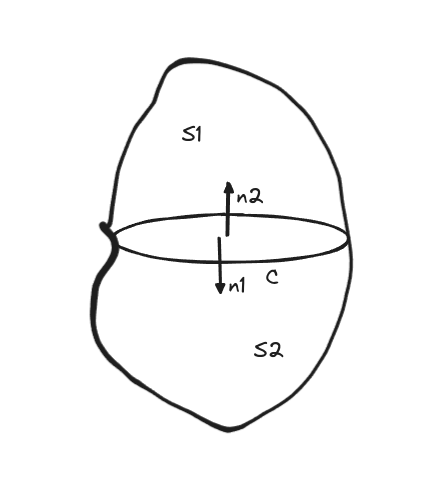
\includegraphics[scale=0.4]{ch1-26.png}
    \end{center}
    Then we can apply Stokes Theorem for both surfaces as
    \begin{align*}
        \int_{S_1} \curl \bm{A} \cdot d\bm{S} &= -\int_{C} \bm{A}\cdot d\bm{l}\\
        \int_{S_2} \curl \bm{A} \cdot d\bm{S} &= \int_{C} \bm{A}\cdot d\bm{l}
    \end{align*}
    Where we added a minus sign to the first equation because the normal
    unit vector $\bm{\hat{n}_1}$ has the opposite direction to $\bm{\hat{n}_2}$.
    Therefore we see that
    \begin{align*}
        \int_{S} \curl \bm{A} \cdot d\bm{S}
        &= \int_{S_1} \curl \bm{A} \cdot d\bm{S}
        + \int_{S_2} \curl \bm{A} \cdot d\bm{S}\\
        &= -\int_{C} \bm{A}\cdot d\bm{l}
        + \int_{C} \bm{A}\cdot d\bm{l}\\
        &= 0
    \end{align*}
\end{proof}
\cleardoublepage
\begin{proof}{\textbf{27.}}
    Let $S$ be a closed surface and $V$ the volume contained in it.
    Also, let $\bm{\Phi}$ be any scalar field and let $\bm{C}$ be a
    constant vector, then we see because of Problem 19 (b) that
    \begin{align*}
        \div (\bm{\Phi C}) &= \bm{\Phi} \div\bm{C} + \bm{C} \cdot \gradient \bm{\Phi}\\
            &= \bm{C} \cdot \gradient \bm{\Phi}
    \end{align*}
    Where we used that $\div\bm{C} = 0$ since $\bm{C}$ is a constant vector.
    Then applying Gauss Theorem to our vector field $\bm{\Phi C}$ we see that
    \begin{align*}
        \int_V \div(\bm{\Phi C}) d\bm{V} &= \int_S (\bm{\Phi C}) \cdot d\bm{S}\\
        \int_V \bm{C}\cdot\gradient\bm{\Phi} d\bm{V}
        &= \int_S (\bm{\Phi C}) \cdot d\bm{S}\\
        \bm{C}\cdot \int_V \gradient\bm{\Phi} d\bm{V}
        &= \bm{C}\cdot\int_S \bm{\Phi} d\bm{S}\\
        \bm{C}\cdot \bigg(\int_V \gradient\bm{\Phi} d\bm{V}
        - \int_S \bm{\Phi} d\bm{S}\bigg)
        &= 0
    \end{align*}
    Finally, since this must hold for any constant vector $\bm{C}$ then it
    could happen that the vector $\bm{C}$ is not perpendicular to
    $\int_V \gradient\bm{\Phi} d\bm{V} - \int_S \bm{\Phi} d\bm{S}$
    so it must happen that
    $$\int_V \gradient\bm{\Phi} d\bm{V} = \int_S \bm{\Phi} d\bm{S}$$
\end{proof}
\cleardoublepage
\begin{proof}{\textbf{28.}}
    Let $S$ be an open surface and $C$ its boundary.
    Also, let $\bm{\Phi}$ be any scalar field and let $\bm{C}$ be a
    constant vector, then we see because of Problem 19 (c) that
    \begin{align*}
        \curl (\bm{\Phi C}) &= \bm{\Phi} \curl\bm{C}
            - \bm{C} \times \gradient \bm{\Phi}\\
            &= - \bm{C} \times \gradient \bm{\Phi}
    \end{align*}
    Where we used that $\curl\bm{C} = 0$ since $\bm{C}$ is a constant vector.
    Then applying Stoke's Theorem to our vector field $\bm{\Phi C}$ we see that
    \begin{align*}
        \int_S (\curl(\bm{\Phi C}))\cdot d\bm{S}
        &= \int_C (\bm{\Phi C}) \cdot d\bm{l}\\
        \int_S (- \bm{C} \times \gradient \bm{\Phi}) \cdot d\bm{S}
        &= \bm{C} \cdot \int_C \bm{\Phi} d\bm{l}\\
        \int_S - \bm{C} \cdot (\gradient \bm{\Phi} \times d\bm{S})
        &= \bm{C} \cdot \int_C \bm{\Phi} d\bm{l}\\
        \bm{C} \cdot \int_S - (\gradient \bm{\Phi} \times d\bm{S})
        &= \bm{C} \cdot \int_C \bm{\Phi} d\bm{l}\\
        \bm{C}\cdot \bigg(
            -\int_S \gradient \bm{\Phi} \times d\bm{S}
            - \int_C \bm{\Phi} d\bm{l}
        \bigg) &= 0
    \end{align*}
    Where we used the triple product property that
    $(\bm{a} \times \bm{b}) \cdot \bm{c} = \bm{a} \cdot(\bm{b} \times \bm{c})$.
 
    Finally, since this must hold for any constant vector $\bm{C}$ then it
    could happen that the vector $\bm{C}$ is not perpendicular to
    $-\int_S \gradient \bm{\Phi} \times d\bm{S} - \int_C \bm{\Phi} d\bm{l}$
    so it must happen that
    $$-\int_S \gradient \bm{\Phi} \times d\bm{S} = \int_C \bm{\Phi} d\bm{l}$$
\end{proof}
\cleardoublepage
\begin{proof}{\textbf{29.}}
    We know that $\laplacian = \div\gradient$ so we can write
    the left-hand side of the equation as
    \begin{align*}
        \int_V \laplacian\frac{1}{|\bm{x}|} d\bm V
        =\int_V \div(\gradient \frac{1}{|\bm{x}|}) d\bm V
    \end{align*}
    By applying Gauss' Theorem we get that
    \begin{align*}
        \int_V \laplacian\frac{1}{|\bm{x}|} d\bm V 
        = \int_V \div(\gradient \frac{1}{|\bm{x}|}) d\bm V
        &= \int_S \gradient \frac{1}{|\bm{x}|} d\bm S
    \end{align*}
    Now considering a sphere centered on the origin and working
    with spherical coordinates, we can write the above equation as
    \begin{align*}
        \int_V \laplacian\frac{1}{|\bm{x}|} d\bm V
        &= \int_S -\frac{1}{r^2} d\bm S
    \end{align*}
    Here we used that the distance from the origin to a point in
    the sphere surface in spherical coordinates is given by $|\bm{x}| = r$
    and hence $\gradient 1/r = -1/r^2$.

    On the other hand, the surface element in spherical coordinates is
    given by $d\bm{S} = r^2 \sin\theta d\theta d\phi$ so integrating along the
    entire sphere surface we get that
    \begin{align*}
        \int_V \laplacian\frac{1}{|\bm{x}|} d\bm V
        &= -\int_0^{2\pi}\int_0^\pi \bigg(\frac{1}{r^2}\bigg)
        r^2 \sin\theta~d\theta d\phi\\
        &= -\int_0^{2\pi}\int_0^\pi \sin\theta~d\theta d\phi\\
        &= -\int_0^{2\pi} \big[-\cos\theta\big]_0^\pi~d\phi\\
        &= -\int_0^{2\pi} 2~d\phi\\
        &= -4\pi
    \end{align*}
\end{proof}
\cleardoublepage
\begin{proof}{\textbf{30.}}
    Let $S$ be a closed surface and $V$ the volume contained in it.
    Also, let $\bm{A}$ be any vector field and let $\bm{B}$ be a
    constant vector, then we see because of Problem 20 (a) that
    \begin{align*}
        \div (\bm{B} \times \bm{A}) &= \bm{A} \cdot (\curl\bm{B})
            - \bm{B} \cdot (\curl\bm{A}) \\
            &= - \bm{B} \cdot (\curl\bm{A})
    \end{align*}
    Where we used that $\curl\bm{B} = 0$ since $\bm{B}$ is a constant vector.
    Then applying Gauss's Theorem to our vector field $\bm{B \times A}$
    we see that
    \begin{align*}
        \int_V \div (\bm B\times \bm A)~d\bm{V}
        &= \int_S (\bm B\times \bm A)\cdot d\bm{S}\\
        \int_V (- \bm{B} \cdot (\curl\bm{A}))~d\bm{V}
        &= \int_S \bm B \cdot( \bm A \times d\bm{S})\\
        \bm{B} \cdot \int_V -(\curl\bm{A})~d\bm{V}
        &= \bm{B} \cdot \int_S  \bm A \times d\bm{S}\\
        \bm{B} \cdot\bigg(
            -\int_V \curl\bm{A}~d\bm{V} -\int_S  \bm A \times d\bm{S}
        \bigg) &= 0
    \end{align*}
    Finally, since this must hold for any constant vector $\bm{B}$ then it
    could happen that the vector $\bm{B}$ is not perpendicular to
    $-\int_V\curl\bm{A}~d\bm{V} -\int_S  \bm A \times d\bm{S}$
    so it must happen that
    \begin{align*}
        \int_V \curl\bm{A}~d\bm{V}
        &= -\int_S  \bm A \times d\bm{S}\\
    \end{align*}
\end{proof}
\cleardoublepage
\begin{proof}{\textbf{32.}}
    Let $\bm{j} = C(xr\hatx + yr\haty)$ or in cartesian coordinates
    $$\bm{j} = C(x\sqrt{x^2 + y^2 + z^2}~\hatx + y\sqrt{x^2 + y^2 + z^2}~\haty)$$
    So $\div \bm{j}$ is given by
    \begin{align*}
        \div \bm{j} &= \partialderivative{j_x}{x} + \partialderivative{j_y}{y}\\
        &= C\frac{2x^2 + y^2 + z^2}{\sqrt{x^2 + y^2 + z^2}}
        + C\frac{x^2 + 2y^2 + z^2}{\sqrt{x^2 + y^2 + z^2}}\\
        &= \frac{C(3(x^2 + y^2) + 2z^2)}{\sqrt{x^2 + y^2 + z^2}}
    \end{align*}
    Or in spherical coordinates
    \begin{align*}
        \div \bm{j} &= \frac{C(3(r^2 - z^2) + 2z^2)}{r}\\
        &= \frac{C(3r^2 - z^2)}{r}\\
        &= \frac{C(3r^2 - r^2\cos^2\theta)}{r}\\
        % &= C(3r - r\cos^2\theta)\\
        &= Cr(3 - \cos^2\theta)
    \end{align*}
    On the other hand, from the charge conservation proof we see that
    \begin{align*}
        \int \div \bm{j}~d\bm{V} = \text{(rate of outflow of charge from V)}
    \end{align*}
    So we compute the rate of change of the electric charge in the spherical
    region bounded by $r = R$ as follows
    \begin{align*}
        \int \div \bm{j}~d\bm{V}
        &= \int_0^{2\pi} \int_0^\pi \int_0^R (Cr(3 - \cos^2\theta))r^2\sin\theta~drd\theta d\phi\\
        &= C\int_0^{2\pi} \int_0^\pi \int_0^R r^3(3 - \cos^2\theta)\sin\theta~drd\theta d\phi\\
        &= C\int_0^{2\pi} \int_0^\pi \bigg[\frac{r^4}{4}\bigg]_0^R(3 - \cos^2\theta)\sin\theta~d\theta d\phi\\
        &= \frac{CR^4}{4}\int_0^{2\pi} \int_0^\pi (2 + \sin^2\theta)\sin\theta~d\theta d\phi\\
        &= \frac{CR^4}{4}\int_0^{2\pi} \int_0^\pi 2\sin\theta + \sin^3\theta~d\theta d\phi
    \end{align*}
    Where we used that $3 - \cos^2\theta = 2 + \sin^2\theta$ hence
    \begin{align*}
        \int \div \bm{j}~d\bm{V}
        &= \frac{CR^4}{4}\int_0^{2\pi} \int_0^\pi 2\sin\theta + \sin^3\theta~d\theta d\phi\\
        &= \frac{CR^4}{4}\int_0^{2\pi} \bigg[
            \frac{1}{12}(\cos(3\theta) - 33\cos\theta)
        \bigg]_0^\pi~ d\phi\\
        &= \frac{CR^4}{4}\int_0^{2\pi}
        \frac{1}{12}[(-1 + 33) - (1 - 33)]~ d\phi\\
        &= \frac{CR^4}{4}\int_0^{2\pi} \frac{16}{3}~d\phi\\
        &= \frac{4CR^4}{3}\int_0^{2\pi} ~d\phi\\
        &= \frac{8\pi}{3}CR^4
    \end{align*}
    % Where we used that $\div \bm{j} = 3Cr$.
\end{proof}













\end{document}
